\section{Semiconductor Physics in Equilibrium}

This section introduces the equilibrium physics of semiconductors. It first outlines the formation of allowed and forbidden energy bands and uses this picture to classify materials as conductors, semiconductors, or insulators. It then summarizes charge-carrier statistics and basic transport mechanisms before discussing Schottky and Ohmic metal-semiconductor contacts. Finally, the section introduces the metal-insulator-semiconductor (MIS) capacitor as a key structure for understanding field-effect devices.

\subsection{Energy Bands and Classification of Materials}
In an isolated atom, electrons occupy discrete energy levels. In a solid,
however, a large number of atoms are arranged close to each other. Due to the
interaction between neighboring atoms and the Pauli exclusion principle, the
discrete atomic energy levels split into a large number of closely spaced
states. These states form quasi-continuous energy bands, while energy regions
with no available electronic states are called band gaps~\cite{Kittel2004,Neamen}.

For the description of electrical conduction, the most important bands are the valence band and the conduction band. The valence band is the highest band that is completely or almost completely occupied at low temperature, whereas the
conduction band contains mobile electrons that can contribute to electrical transport. The energy difference between the conduction-band minimum $E_\mathrm{C}$ and the valence-band maximum $E_\mathrm{V}$ is called the band gap,
\begin{equation}
    E_\mathrm{g} = E_\mathrm{C} - E_\mathrm{V}.
\end{equation}
The occupation probability of an electronic state with energy $E$ in thermal equilibrium is described by the Fermi--Dirac distribution
\begin{equation}
    f(E) =
    \frac{1}{1 + \exp\left(\frac{E-E_\mathrm{F}}{k_\mathrm{B}T}\right)},
\end{equation}
where $E_\mathrm{F}$ is the Fermi energy, $k_\mathrm{B}$ is the Boltzmann constant, and $T$ is the absolute temperature. The Fermi energy represents the electrochemical potential of the electron system in thermal equilibrium. At $E=E_\mathrm{F}$, the occupation probability is equal to $1/2$~\cite{Neamen}.

Depending on their electrical resistivity and band structure, solids can be classified into metals, semiconductors, and insulators. Semiconductors typically have a finite band gap below about \SI{4}{\electronvolt}, whereas insulators
usually have larger band gaps. The boundaries between these classes are not perfectly sharp, since the resistivity depends on temperature, purity, crystal structure and doping concentration. Nevertheless, the orders of magnitude listed
in Table~\ref{tab:material_classification} are useful for a qualitative classification~\cite{Kittel2004,Neamen}.

\begin{table}[h]
    \centering
    \begin{tabular}{p{3cm} p{4cm} p{3cm} p{3.4cm}}
        \hline
        \textbf{Material class} &
        \textbf{Typical resistivity $\rho$} &
        \textbf{Band gap $E_\mathrm{g}$} &
        \textbf{Examples} \\
        \hline
        Metal &
        $10^{-8}$--$10^{-6}\,\Omega\,\mathrm{m}$ &
        Small or overlap  &
        Cu, Ag, Au, Al \\

        Semiconductor &
        $10^{-4}$--$10^{7}\,\Omega\,\mathrm{m}$ &
        $0<E_\mathrm{g}<\SI{4}{\electronvolt}$ &
        Si, Ge, GaAs, pentacene, C8-BTBT \\

        Insulator &
        $>10^{7}\,\Omega\,\mathrm{m}$, often up to
        $10^{16}\,\Omega\,\mathrm{m}$ or higher &
        $E_\mathrm{g}>\SI{4}{\electronvolt}$ &
        SiO$_2$, glass, Al$_2$O$_3$, polystyrene \\
        \hline
    \end{tabular}
    \caption{Classification of materials according to typical electrical
    resistivity and approximate band-gap range.}
    \label{tab:material_classification}
\end{table}

In metals, electrons can easily occupy nearby empty states because the Fermi level lies inside an allowed energy band. Therefore, metals show high electrical conductivity and low resistivity~\cite{Kittel2004,Neamen}.

In semiconductors, the band gap is finite but sufficiently small that charge carriers can be generated thermally or by external excitation. Electrons in the conduction band and holes in the valence band can both contribute to charge
transport. In addition, the carrier density can be controlled by doping or by an external electric field, which is the physical basis of field-effect devices~\cite{Neamen}.

In insulators, the band gap is large and the number of thermally generated charge carriers at room temperature is negligible. Therefore, their electrical resistivity is very high~\cite{Kittel2004,Neamen}.

\begin{figure}[h]
    % \vspace{-\baselineskip}
    \centering
    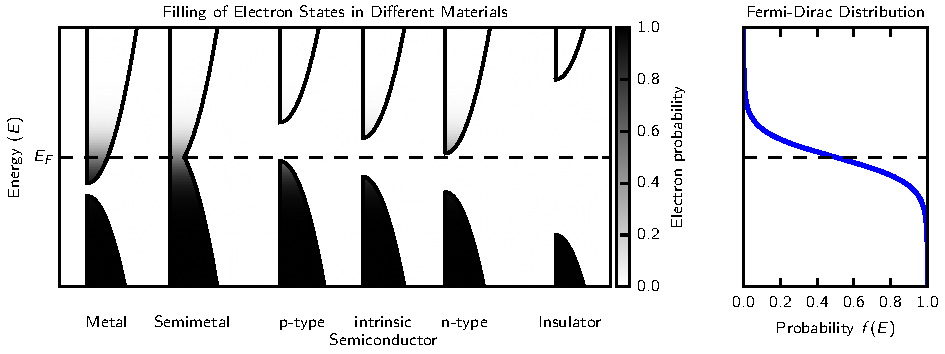
\includegraphics[scale=1]{figures/band_diagram.pdf}
    \caption[Electron occupancy of allowed energy bands in metals, semimetals, semiconductors, and insulators at temperature $T>0~\si{K}$]{Electron occupancy of allowed energy bands in metals, semimetals, semiconductors, and insulators at temperature $T>0~\si{K}$. Shading indicates Fermi--Dirac occupation from filled states (black) to empty states (white).}
    \label{fig:energy_band_occupancy}
\end{figure}

The same terminology is often used for organic semiconductors, although the microscopic origin of the relevant electronic states is different. Instead of
ideal crystal bands, organic semiconductors are commonly described in terms of
molecular orbitals. The highest occupied molecular orbital (HOMO) is analogous
to the valence band, while the lowest unoccupied molecular orbital (LUMO) is
analogous to the conduction band. In $p$-type organic semiconductors such as C8-BTBT,
charge transport is mainly associated with holes in HOMO-derived transport
states~\cite{Bruetting2005}.


\subsection{Statistics and Transport Phenomena of Charge Carriers}

The electrical conductivity of a semiconductor is determined by the number of
mobile charge carriers and by their ability to move through the material. The
mobile carriers are electrons in the conduction band and holes in the valence
band. Their concentrations are obtained from the density of available electronic
states and from the occupation probability of these states~\cite{Neamen}.

The electron density in the conduction band is obtained by multiplying the
available density of states by the occupation probability and integrating over
all conduction-band energies. For a non-degenerate semiconductor, this expression
can be written in the Boltzmann approximation as~\cite{Neamen}
\begin{equation}
    n = \int_{E_\mathrm{C}}^{\infty} D_\mathrm{C}(E) f(E) \, \mathrm{d}E
    \approx N_\mathrm{C}
    \exp\left(-\frac{E_\mathrm{C}-E_\mathrm{F}}{k_\mathrm{B}T}\right),
\end{equation}
where $D_\mathrm{C}(E)$ is the density of states in the conduction band and
$N_\mathrm{C}$ is the effective density of states in the conduction band.
Correspondingly, the hole density in the valence band is
\begin{equation}
    p = \int_{-\infty}^{E_\mathrm{V}} D_\mathrm{V}(E) \left[1-f(E)\right]
    \, \mathrm{d}E
    \approx N_\mathrm{V}
    \exp\left(-\frac{E_\mathrm{F}-E_\mathrm{V}}{k_\mathrm{B}T}\right),
\end{equation}
where $D_\mathrm{V}(E)$ is the density of states in the valence band and
$N_\mathrm{V}$ is the effective density of states in the valence band. The factor
$1-f(E)$ describes the probability that an electronic state in the valence band
is empty. These equations show that the electron density increases when the
Fermi level moves closer to the conduction band, whereas the hole density
increases when the Fermi level moves closer to the valence band~\cite{Neamen}.

For an intrinsic semiconductor, the electron and hole concentrations are equal,
\begin{equation}
    n = p = n_i =\sqrt{N_\mathrm{C}N_\mathrm{V}}
    \exp\left(-\frac{E_\mathrm{g}}{2k_\mathrm{B}T}\right),
\end{equation}
where $n_i$ is the intrinsic carrier concentration~\cite{Neamen}.

In thermal equilibrium, the product of electron and hole density is given by the
mass action law~\cite{Neamen}
\begin{equation}
    np = n_i^2 .
\end{equation}
The carrier concentrations can also be expressed relative to the intrinsic
Fermi level $E_\mathrm{Fi}$~\cite{Neamen},
\begin{equation}
    n = n_i \exp\left(\frac{E_\mathrm{F}-E_\mathrm{Fi}}{k_\mathrm{B}T}\right),
\end{equation}
\begin{equation}
    p = n_i \exp\left(\frac{E_\mathrm{Fi}-E_\mathrm{F}}{k_\mathrm{B}T}\right).
\end{equation}
For parabolic bands and similar effective masses of electron and hole, the
intrinsic Fermi level is approximately
\begin{equation}
    E_\mathrm{Fi} \approx \frac{1}{2}\left(E_\mathrm{V}+E_\mathrm{C}\right),
\end{equation}
which lies close to the middle of the band gap~\cite{Neamen}.

This relation is valid for a non-degenerate semiconductor in thermal
equilibrium. If the semiconductor is doped, the Fermi level shifts away from the
intrinsic level, as illustrated in Figure~\ref{fig:carriers_concentration}. In a
$p$-type semiconductor, acceptor atoms increase the hole concentration and shift
the Fermi level closer to the valence band. For a strongly doped $p$-type
semiconductor with complete ionization of acceptors, the carrier densities are
approximately~\cite{Neamen}
\begin{equation}
    p \approx N_\mathrm{A}, \qquad n = \frac{n_i^2}{p} \ll p.
\end{equation}
In an $n$-type semiconductor, donor atoms increase the electron concentration
and shift the Fermi level closer to the conduction band. Similarly, for a
strongly doped $n$-type semiconductor with complete ionization of donors, the
carrier densities are approximately~\cite{Neamen}
\begin{equation}
    n \approx N_\mathrm{D}, \qquad p = \frac{n_i^2}{n} \ll n.
\end{equation}

\begin{figure}[h]
    % \vspace{-\baselineskip}
    \centering
    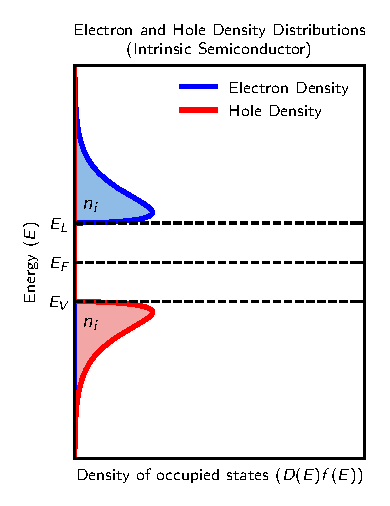
\includegraphics[scale=1]{figures/intrinsic_density}
    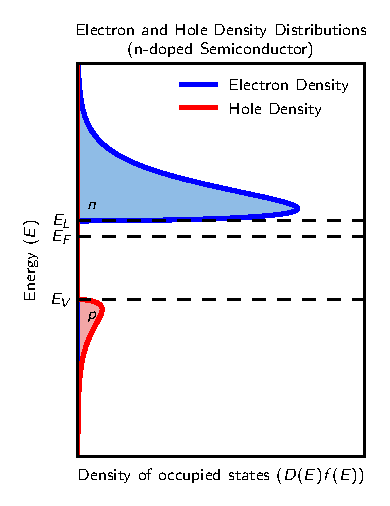
\includegraphics[scale=1]{figures/doped_density}
    \caption[Carrier concentrations in intrinsic (left) and $n$-type (right) semiconductors]{Carrier concentrations in intrinsic (left) and p-type (right) semiconductors. In an intrinsic semiconductor, electron and hole concentrations are equal, $n=p=n_i$. Doping shifts the Fermi level and changes the majority and minority carrier densities.}
    \label{fig:carriers_concentration}
\end{figure}

Charge transport in semiconductors is caused by drift and diffusion. In the
Drude model, mobile charge carriers are accelerated by an electric field and
lose momentum through scattering events characterized by an average relaxation
time $\tau$. This leads to a drift velocity proportional to the electric field,
with the proportionality described by the mobility, $\mu = q\tau/m^*$, where
$m^*$ is the effective mass~\cite{Neamen}. Drift transport therefore occurs
when an electric field acts on mobile charge carriers. The electric field is
related to the electrostatic potential by
\begin{equation}
    \mathbf{E} = - \nabla \varphi .
\end{equation}
The spatial distribution of charge carriers is coupled to the electrostatic
potential through Poisson's equation~\cite{Neamen},
\begin{equation}
    \nabla \cdot \left(-\epsilon_0 \epsilon_r \nabla \varphi\right)
    = \rho
    = e \left(p - n + N_\mathrm{D}^{+} - N_\mathrm{A}^{-}\right),
\end{equation}
where $\epsilon_0$ is the vacuum permittivity, $\epsilon_r$ is the relative
permittivity, $e$ is the elementary charge, and $N_\mathrm{D}^{+}$ and
$N_\mathrm{A}^{-}$ are the ionized donor and acceptor concentrations,
respectively.
The quantities $\mu_n$ and $\mu_p$ denote the electron and hole mobilities,
which describe how fast charge carriers move in response to an applied electric
field. Diffusion transport occurs when the carrier concentration is spatially
inhomogeneous, causing charge carriers to move from regions of high
concentration to regions of low concentration. Combining drift and diffusion,
the total current density can be written as~\cite{Neamen}
\begin{equation}
    \mathbf{J} = q \left(n\mu_n + p\mu_p\right)\mathbf{E}
    + q \left(D_n\nabla n - D_p\nabla p\right).
\end{equation}
In steady state, charge conservation requires that the current density is
divergence-free,
\begin{equation}
    \nabla \cdot \mathbf{J} = 0.
\end{equation}
For a homogeneous semiconductor, where concentration gradients can be neglected,
the current density is dominated by drift. The electrical conductivity is then
\begin{equation}
    \sigma = q \left(n\mu_n + p\mu_p\right).
\end{equation}
Compared with an intrinsic semiconductor, a doped semiconductor usually has a
much larger conductivity because doping increases the majority carrier
concentration by many orders of magnitude. Since the conductivity is
proportional to the carrier density, this increase can dominate even if the
mobility is reduced by impurity scattering~\cite{Neamen}. For a $p$-type
organic semiconductor such as C8-BTBT~\cite{Bruetting2005}, in which holes are
the majority carriers and the electron contribution is negligible, this
simplifies to
\begin{equation}
    \sigma \approx q p \mu_p .
\end{equation}
In thermal equilibrium, no net current flows. This does not mean that electrons
and holes are immobile. Rather, microscopic motion is still present, but drift
and diffusion currents balance each other exactly. This balance is expressed by
the Einstein relation~\cite{Neamen},
\begin{equation}
    \frac{D_n}{\mu_n} = \frac{D_p}{\mu_p}
    = \frac{k_\mathrm{B}T}{q}.
\end{equation}
In organic semiconductors, the same macroscopic quantities, such as carrier
density, mobility and conductivity, are used to describe charge transport.
However, the microscopic transport mechanisms can differ from those in ideal
inorganic crystals. Due to weak van der Waals coupling, energetic disorder,
grain boundaries and trap states, charge transport in organic thin films may
involve both band-like motion and hopping between localized states. In
polycrystalline organic semiconductors, grain boundaries and traps can reduce
the effective mobility measured over macroscopic distances. Therefore, the
mobility extracted from electrical measurements should be understood as an
effective transport parameter of the investigated thin film~\cite{Bruetting2005}.



\subsection{Metal-Semiconductor Contacts}

Metal--semiconductor contacts determine how efficiently carriers enter and leave
the semiconductor. Even if transport in the channel is described by drift and
diffusion, the measured current can be limited by injection barriers at the
electrodes. The two limiting cases are rectifying Schottky contacts and nearly
barrier-free Ohmic contacts~\cite{Neamen,ElKareh2015RectifyingOhmicContacts}.

Before contact, the metal and semiconductor have independent Fermi levels. After
contact, charge transfer aligns the Fermi levels and bends the semiconductor
bands near the interface, as shown in
Figure~\ref{fig:schottky_barrier_before_after_contact}. For a $p$-type
semiconductor, a low metal work function relative to the semiconductor work
function depletes holes at the interface and produces a Schottky barrier. In the
ideal Schottky--Mott picture this rectifying case is expected when
\begin{equation}
    \phi_\mathrm{m} < \phi_\mathrm{s},
\end{equation}
and the approximate hole barrier height is
\begin{equation}
    e\phi_\mathrm{B} = E_\mathrm{g} - e(\phi_\mathrm{m} - \chi).
\end{equation}
Thus, higher-work-function electrodes reduce the barrier for hole injection,
whereas lower-work-function electrodes increase the contact resistance~\cite{Neamen}.

\begin{figure}[h]
    \centering
    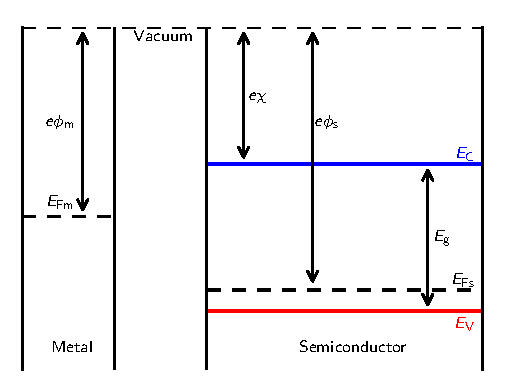
\includegraphics[scale=1]{figures/Schottky-before-contact}
    \hfill
    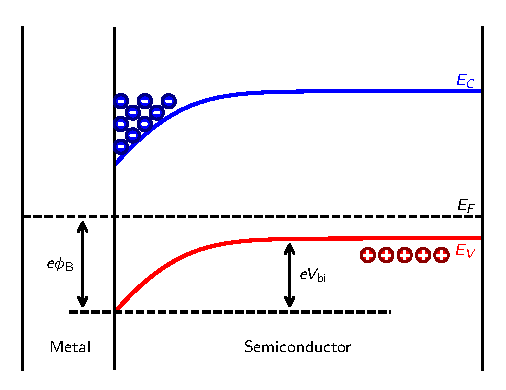
\includegraphics[scale=1]{figures/Schottky-after-contact}

    \caption[Schottky barrier formation at a metal--$p$-type semiconductor
    contact]{Schottky barrier formation at a metal--$p$-type semiconductor
    contact. Band alignment of a metal and a $p$-type semiconductor before (left) and
    after contact (right). Fermi-level alignment causes band bending in the semiconductor
    and can form a Schottky barrier for hole transport.}
    \label{fig:schottky_barrier_before_after_contact}
\end{figure}

For C8-BTBT devices, the HOMO or ionization energy is about
\SI{5.4}{\electronvolt}, while chromium has a lower work function of roughly
\SI{4.5}{\electronvolt}. A direct Cr/C8-BTBT interface is therefore expected to
form a hole-injection barrier. High-work-function MoO$_x$ or MoO$_3$ interlayers
can reduce this barrier and are commonly used to improve hole injection in
organic field-effect transistors~\cite{Michaelson1977WorkFunctionElements,Wang2017LowVoltageC8BTBT,Greiner2013ThinFilmMetalOxides,Ablat2019OxideMetalBilayerElectrodes}.

The band diagram also explains the bias dependence of contact behavior. In a
Schottky contact, band bending creates a depletion region and a bias-dependent
barrier: forward bias lowers the barrier, while reverse bias widens the
depletion region and suppresses injection. In contrast, an Ohmic contact has a
small or tunnelable injection barrier, so the current--voltage relation is
approximately linear at small bias. For $p$-type semiconductors this is favored
when $\phi_\mathrm{M} \gtrsim \phi_\mathrm{S}$, although interface dipoles,
chemical reactions, disorder, and traps often modify the ideal work-function
picture~\cite{Neamen,ElKareh2015RectifyingOhmicContacts}.

Several microscopic processes can contribute to carrier transfer across the
interface. If the barrier is relatively high and wide, carriers must be
thermally excited over it; this thermionic-emission process is strongly
temperature dependent and gives rectifying behavior. Once carriers enter the
semiconductor, they are transported away from the interface by drift in the local
electric field and by diffusion caused by carrier-concentration gradients. If
the barrier is thin, for example due to strong band bending, heavy doping, or an
interfacial oxide, carriers can also tunnel through it. Real organic contacts
often combine these mechanisms with hopping through localized interfacial states,
so the observed contact resistance reflects both the injection barrier and the
near-interface transport region~\cite{Neamen,Bruetting2005}.

\begin{figure}[h!]
    \centering
    \setlength{\tabcolsep}{3pt}
    \renewcommand{\arraystretch}{1.15}
    \resizebox{\textwidth}{!}{%
    \begin{tabular}{|>{\centering\arraybackslash}m{0.9cm}|>{\centering\arraybackslash}m{0.36\textwidth}|>{\centering\arraybackslash}m{0.36\textwidth}|}
        \hline
        & \footnotesize{\textbf{Schottky contact}} &  \footnotesize{\textbf{Ohmic contact}} \\
        \hline
        \rotatebox{90}{ \footnotesize{\textbf{Thermal equilibrium}}} &
        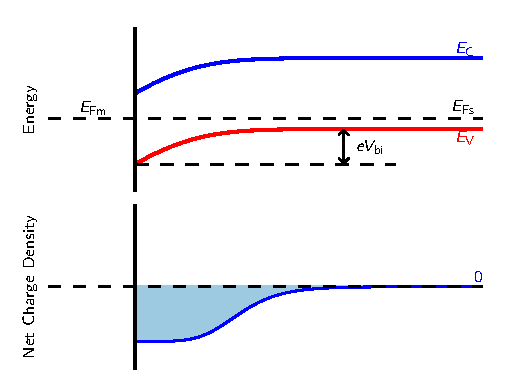
\includegraphics[width=0.36\textwidth]{figures/schottky-00} &
        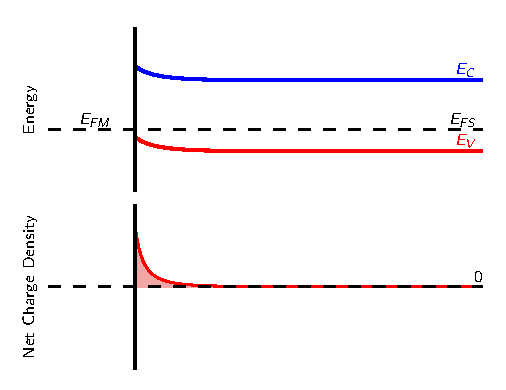
\includegraphics[width=0.36\textwidth]{figures/ohmic-00} \\
        \hline
        \rotatebox{90}{ \footnotesize{\textbf{Forward bias}}} &
        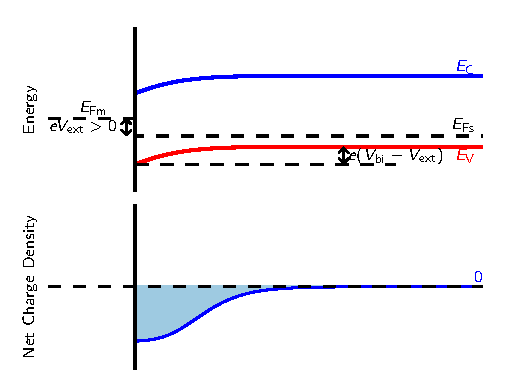
\includegraphics[width=0.36\textwidth]{figures/schottky-01} &
        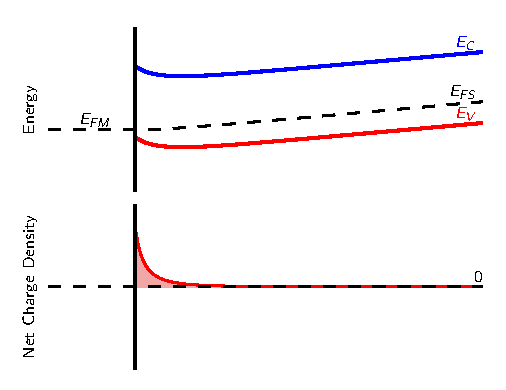
\includegraphics[width=0.36\textwidth]{figures/ohmic-01} \\
        \hline
        \rotatebox{90}{ \footnotesize{\textbf{Reverse bias}}} &
        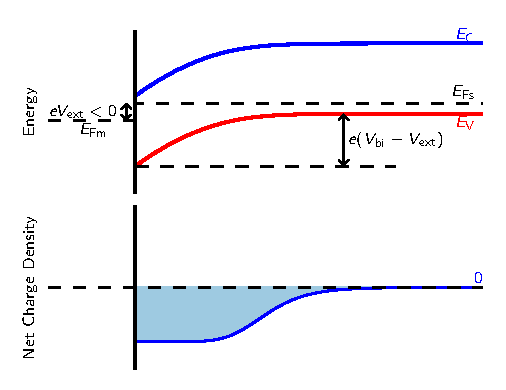
\includegraphics[width=0.36\textwidth]{figures/schottky-02} &
        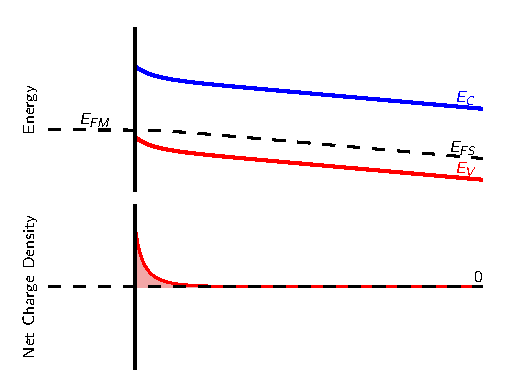
\includegraphics[width=0.36\textwidth]{figures/ohmic-02} \\
        \hline
    \end{tabular}
    }
    \caption[Band diagrams of Schottky and Ohmic contacts for p-type semiconductors]{Band diagrams and
    corresponding net charge-density profiles for metal--semiconductor contacts
    under equilibrium, forward-bias, and reverse-bias conditions.}
    \label{fig:metal_semiconductor_band_diagrams}
\end{figure}

\subsection{Metal-Insulator-Semiconductor Capacitor}

A metal--insulator--semiconductor (MIS) capacitor consists of a metal gate, an
insulating dielectric, and a semiconductor. Because the dielectric blocks direct
DC current, the gate voltage controls the semiconductor mainly through the
electric field across the insulator. This field changes the surface potential and
therefore the carrier density at the semiconductor--insulator interface. The MIS
capacitor is thus the basic electrostatic model for field-effect devices~\cite{Neamen,Hu2010MOSCapacitor}.

In a band diagram, flat-band conditions correspond to nearly horizontal
semiconductor bands and no net space-charge region at the surface. Applying a
gate voltage bends the bands near the interface. For a $p$-type semiconductor,
negative gate bias attracts holes and produces accumulation, while positive gate
bias repels holes and produces depletion. Strong positive bias can lead to
inversion in ideal inorganic semiconductors, but in many $p$-type organic
semiconductors the practically relevant regimes are mainly accumulation and
depletion~\cite{Manda2018OrganicMISCapacitor,Bruetting2005}.

The gate dielectric is described by its geometric area capacitance,
\begin{equation}
    C_\mathrm{i} = \frac{\epsilon_0 \epsilon_\mathrm{i}}{d_\mathrm{i}} ,
\end{equation}
so the induced sheet charge density in accumulation is approximately
\begin{equation}
    p_\text{2D} \approx \frac{C_\mathrm{i}|V_\mathrm{G}-V_\mathrm{T}|}{e}.
\end{equation}
Here $V_\mathrm{T}$ represents threshold voltage, which consists of  flat-band shifts, trap filling, and contact
effects. The MIS picture therefore links gate voltage, band bending, interfacial
carrier density, and field-effect transport in organic semiconductor devices~\cite{Hu2010MOSCapacitor,Manda2018OrganicMISCapacitor}.